%worksheet5.tex
%problem set for the course PandA2 COMS10001 taught at the University of Bristol
%2017 Conor Houghton conor.houghton@bristol.ac.uk

%To the extent possible under law, the author has dedicated all copyright 
%and related and neighboring rights to these notes to the public domain 
%worldwide. These notes are distributed without any warranty. 



\documentclass[11pt,a4paper]{scrartcl}
\typearea{12}
\usepackage{graphicx}
\usepackage{pstricks}
\usepackage{tikz-qtree}
\usepackage{listings}
\usepackage{color}
\usetikzlibrary{positioning}
\newif\ifanswers
%\answerstrue
\answersfalse

\lstset{language=C}
\pagestyle{headings}
\markright{COMS10001 - PandA2 algorithms worksheet 5 - Conor}
\begin{document}
\tikzset{every tree node/.style={minimum width=2em,draw,circle},
  blank/.style={draw=none}, edge from parent/.style= {draw,->, edge
    from parent path={(\tikzparentnode) -- (\tikzchildnode)}}, level
  distance=1.5cm}


\subsection*{Algorithms Worksheet 5}

This week there are two question each worth four marks, there are two
marks for attendance.

\begin{enumerate}

\item  Heapify the list $(15,2,23,19,24,13,8)$.

\ifanswers

\noindent Solution: The key point is you add each item at the next
available slot in the tree and then if it violates the rule that items are smaller than their parent, you swap it upwards until it works. So
\begin{center}
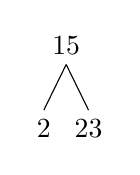
\begin{tikzpicture}
\Tree [.15 2 23 ]
\end{tikzpicture}
\end{center}
gets changed to
\begin{center}
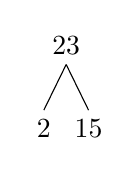
\begin{tikzpicture}
\Tree [.23 2 15 ]
\end{tikzpicture}
\end{center}
Next adding to the next layer
\begin{center}
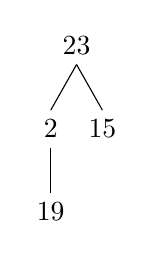
\begin{tikzpicture}
\Tree [.23 [.2 19 ] 15 ]
\end{tikzpicture}
\end{center}
becomes
\begin{center}
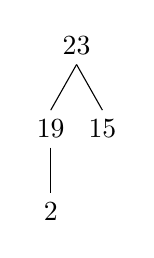
\begin{tikzpicture}
\Tree [.23 [.19 2 ] 15 ]
\end{tikzpicture}
\end{center}
and then
\begin{center}
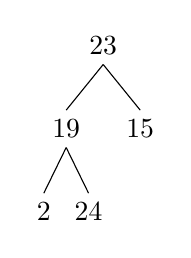
\begin{tikzpicture}
\Tree [.23 [.19 2 24 ] 15 ]
\end{tikzpicture}
\end{center}
goes to
\begin{center}
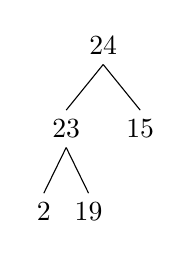
\begin{tikzpicture}
\Tree [.24 [.23 2 19 ] 15 ]
\end{tikzpicture}
\end{center}
Next
\begin{center}
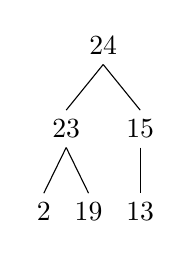
\begin{tikzpicture}
\Tree [.24 [.23 2 19 ] [.15 13 ] ]
\end{tikzpicture}
\end{center}
becomes
\begin{center}
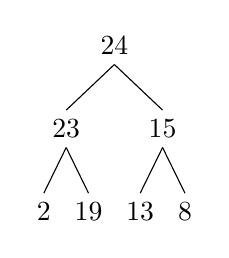
\begin{tikzpicture}
\Tree [.24 [.23 2 19 ] [.15 13 8 ] ]
\end{tikzpicture}
\end{center}
and then it finishes.
\fi

\item Consider the following example code, taken from the wikipedia article on loop invariants:
\begin{lstlisting}[numbers=left]
int max(int n,const int a[]) {
     int m = a[0];
     int i = 1;
     while (i != n) {
         if (m < a[i])
             m = a[i];
         ++i;

     }
     return m;
}
\end{lstlisting}
Explain what is meant by the claim that 
\begin{quote}
\texttt{m} is the maximum
of \texttt{a[0...i-1]} 
\end{quote}
is a loop invariant for this function whose purpose is to find the
maximum in \texttt{a}.

\ifanswers

\noindent Solution: the statement is true at the start in line 3
because \texttt{i=1} and \texttt{m=a[0]} which is trivially the
maximum; if the statement is true at the start
of the loop then the new element is bigger than all the previous ones, in which \texttt{m} is set equal the new element, or the maximum remains the same, either way the invariant remains true at the end and if it is true when \texttt{i=n} then the algorithm has succeeded.
\fi


\end{enumerate}

\end{document}
